\documentclass[10pt,twocolumn,a4paper]{article}
\usepackage[utf8]{vietnam}
\usepackage[top=1.5cm,bottom=1.6cm,left=1.4cm,right=1.4cm,columnsep=0.55cm]{geometry}
\usepackage{amsmath,amssymb}
\usepackage{booktabs,multirow,tabularx,array}
\usepackage{graphicx}
\usepackage[font=footnotesize,labelfont=bf,skip=3pt]{caption}
\usepackage{subcaption}
\usepackage{enumitem}
\usepackage{xcolor}
\usepackage{float}
\usepackage{placeins}
\usepackage{microtype}
\usepackage[colorlinks=true,linkcolor=blue!60!black,citecolor=blue!60!black,urlcolor=blue!60!black]{hyperref}
\usepackage{titlesec}

\renewcommand{\topfraction}{0.92}
\renewcommand{\bottomfraction}{0.85}
\renewcommand{\textfraction}{0.06}
\renewcommand{\floatpagefraction}{0.82}
\renewcommand{\dbltopfraction}{0.92}
\renewcommand{\dblfloatpagefraction}{0.82}
\setcounter{topnumber}{3}
\setcounter{dbltopnumber}{3}
\setcounter{totalnumber}{5}

\setlist[itemize]{nosep,leftmargin=1.2em,topsep=2pt}
\setlist[enumerate]{nosep,leftmargin=1.4em,topsep=2pt}
\setlength{\textfloatsep}{6pt plus 2pt minus 2pt}
\setlength{\floatsep}{5pt plus 2pt minus 2pt}
\setlength{\intextsep}{5pt plus 2pt minus 2pt}
\titlespacing*{\section}{0pt}{7pt plus 2pt minus 1pt}{3pt}
\titlespacing*{\subsection}{0pt}{5pt plus 1pt minus 1pt}{2pt}

\title{\vspace{-0.8cm}\textbf{\Large Đánh Giá Tác Động Của Các Phương Pháp Xử Lý Ảnh Cổ Điển Lên Mô Hình Phân Loại Tổn Thương Da HAM10000 Sử Dụng Mạng Nơ-ron Tích Chập}}
\author{
\normalsize\textbf{Nguyễn Trung Nam (B23DCVT299), Phan Nguyễn Việt Dũng (B23DCCN210),}\\
\normalsize\textbf{Lê Duy Anh (B23DCCN026), Đinh Khánh Sơn (B23DCDT223), Đào Phạm Bích Ngọc (B23DCVT308)}\\
\small Học phần Xử lý ảnh -- Khoa Trí tuệ Nhân tạo, Học viện Công nghệ Bưu chính Viễn thông (PTIT)\\
\small Mã nguồn \& thực nghiệm tái lập: \url{https://github.com/VietDunghere/Image-Processing}
}
\date{\vspace{-0.3cm}\small Tháng 11 năm 2026}

\begin{document}
\maketitle

\begin{abstract}
\noindent Trong thị giác máy tính hiện đại, mạng tích chập sâu (CNN) thường được huấn luyện trực tiếp trên ảnh thô, đặt ra câu hỏi liệu các phép nâng cao chất lượng ảnh cổ điển còn mang lại lợi ích thực chất hay không. Nghiên cứu này thực hiện đánh giá thực nghiệm có kiểm soát chặt chẽ trên bộ dữ liệu soi da thực tế \textbf{HAM10000} ($10\,015$ ảnh dermoscopy $600{\times}450$ thuộc $7\,470$ tổn thương, 7 lớp bệnh mất cân bằng $58{,}3$ lần). Trước hết, chúng tôi xây dựng bộ 7 chỉ số định lượng bám sát Chương 3, 4, 5, 7 của học phần để kiểm định các vấn đề chất lượng ảnh và phát hiện 6 hiện tượng có bằng chứng thống kê (lông che phủ $10{,}1\%$, nhiễu Gauss nhẹ $7{,}3\%$, tương phản thấp $4{,}3\%$, viền tối ống soi $3{,}5\%$, quá sáng bạc màu $3{,}0\%$, chiếu sáng lệch $2{,}5\%$), đồng thời bác bỏ nhiễu muối--tiêu và quá tối. Trên phân chia chống rò rỉ theo \texttt{lesion\_id} và cấu hình đóng băng có lấy mẫu cân bằng WRS qua 3 seed độc lập, chúng tôi so sánh 3 kiến trúc (\texttt{ResNet-18}, \texttt{EfficientNet-B0}, \texttt{MobileNetV3-Small}) và đánh giá 16 cấu hình tiền xử lý trên \texttt{ResNet-18} (baseline đạt test macro-F1 $0{,}6941 \pm 0{,}0160$). Kết quả cho thấy \textbf{0/16 cấu hình cải thiện rõ} macro-F1 trên validation; đặc biệt cân bằng lược đồ toàn cục (\texttt{hist\_eq\_L}, $\Delta=$-$0{,}1106$) và giãn tuyến tính (\texttt{stretch\_L\_1\_99}, $\Delta=$-$0{,}0786$) làm giảm mạnh hiệu năng do lệch màu $\Delta E_{76}$ và khuếch đại nhiễu, còn xóa lông đại trà (\texttt{hair\_bh17}) inpaint nhầm mạng sắc tố của u hắc tố (\texttt{mel}). Phân tích sâu 4 tầng (ảnh, mức nền đổi nhãn, stress test suy giảm tổng hợp và Grad-CAM) lý giải trọn vẹn cơ chế này và dẫn tới đề xuất \textbf{pipeline hai nhánh}: nhánh Kiểm tra chất lượng (QC) gắn cờ cảnh báo song song với nhánh phân loại CNN trên ảnh gốc, triển khai trực quan trên ứng dụng Streamlit.
\end{abstract}

\section{Giới thiệu và Câu hỏi nghiên cứu}
\textbf{Bài toán và động cơ.} Phân loại đa lớp ảnh tổn thương da (7 lớp: \texttt{akiec, bcc, bkl, df, mel, nv, vasc}) trên tập dữ liệu thực tế HAM10000~\cite{tschandl2018ham10000} đối mặt với ba trở ngại lớn: (i) nhiễu và sai lệch thu nhận ảnh từ máy soi da (viền đen cơ học, phản xạ lóa của gel/LED, sợi lông che khuất, độ tương phản thấp); (ii) mất cân bằng lớp gay gắt ($6\,705$ ảnh \texttt{nv} so với $115$ ảnh \texttt{df}); và (iii) một \texttt{lesion\_id} có nhiều ảnh chụp làm phát sinh nguy cơ rò rỉ dữ liệu nếu chia ngẫu nhiên theo ảnh. Mục tiêu của đồ án \emph{không} phải tối ưu hóa điểm số SOTA bằng mọi giá, mà tuân thủ phương pháp luận \textbf{lập luận $\rightarrow$ thực nghiệm kiểm soát biến $\rightarrow$ đánh giá trung thực}, trong đó kết quả âm (``không cải thiện'' hoặc ``làm tệ đi'') vẫn là đóng góp khoa học hợp lệ.

\textbf{Câu hỏi nghiên cứu (RQ) và ánh xạ học phần.} Nghiên cứu giải quyết 4 câu hỏi: \textbf{RQ1} -- Tập ảnh có những vấn đề chất lượng nào có bằng chứng thống kê và liên hệ thế nào với lỗi CNN? \textbf{RQ2} -- Từng phương pháp xử lý cổ điển (áp đại trà hoặc có điều kiện) có tạo chênh lệch macro-F1 vượt ngưỡng dao động giữa các seed không? \textbf{RQ3} -- Tác động thực sự diễn ra ở tầng nào (chỉ số ảnh, đổi nhãn dự đoán, stress test suy giảm nặng hay vùng chú ý Grad-CAM)? \textbf{RQ4} -- Ghép nối nhiều bước xử lý và lựa chọn kiến trúc CNN dẫn tới pipeline cuối ra sao? Toàn bộ công cụ bám sát học phần: \textbf{Chương 3} (lược đồ xám, giãn/cân bằng lược đồ, CLAHE~\cite{zuiderveld1994clahe}, gamma, lọc Gauss/trung vị, khôi phục inpainting Telea~\cite{telea2004inpainting}), \textbf{Chương 4} (không gian HSV và mở rộng sang CIE $L^*a^*b^*$), \textbf{Chương 5} (Sobel, phân ngưỡng Otsu~\cite{otsu1979threshold}), \textbf{Chương 6} (kiểm tra nén JPEG), \textbf{Chương 7} (đóng, mở, giãn, black-hat) và \textbf{Chương 8} (CNN~\cite{he2016resnet,tan2019efficientnet,howard2019mobilenetv3} và Grad-CAM~\cite{selvaraju2017gradcam}).

\section{Dữ liệu, Phân tích chất lượng ảnh (EDA) và Chuẩn bị}
\subsection{Mô tả dữ liệu HAM10000 và Cảnh báo lệch miền}
Bộ dữ liệu gồm $10\,015$ ảnh RGB đồng nhất kích thước $600{\times}450$ từ $7\,470$ \texttt{lesion\_id}~\cite{tschandl2018ham10000}. Nhãn được xác nhận qua 4 phương thức (\texttt{dx\_type}): mô bệnh học \texttt{histo} ($53{,}3\%$), theo dõi số hóa \texttt{follow\_up} ($37{,}0\%$), đồng thuận \texttt{consensus} ($9{,}0\%$) và kính đồng tiêu \texttt{confocal} ($0{,}7\%$) (Hình~\ref{fig:data_wrs}a). Đáng chú ý, toàn bộ $3\,704$ ảnh \texttt{follow\_up} đều thuộc lớp \texttt{nv}, tạo nguy cơ mô hình học dấu vết thiết bị/nguồn chụp (\emph{shortcut learning}). Có $1\,956$ lesion ($26{,}2\%$) chứa $\ge 2$ ảnh (chiếm $44{,}9\%$ tổng số ảnh), bao gồm 2 nhóm trùng byte và 19 cặp gần trùng (aHash $\le 2$ bit) đều nằm trong cùng \texttt{lesion\_id}. Đặc biệt, đây là ảnh \textbf{soi da áp sát (dermoscopy)} chứ không phải ảnh chụp bằng điện thoại thông thường; do đó mọi thử nghiệm ngoài tập bằng ảnh điện thoại ở phần demo chỉ mang ý nghĩa minh họa định tính giai đoạn xử lý, không dùng để chẩn đoán y khoa.

\begin{figure}[t]
    \centering
    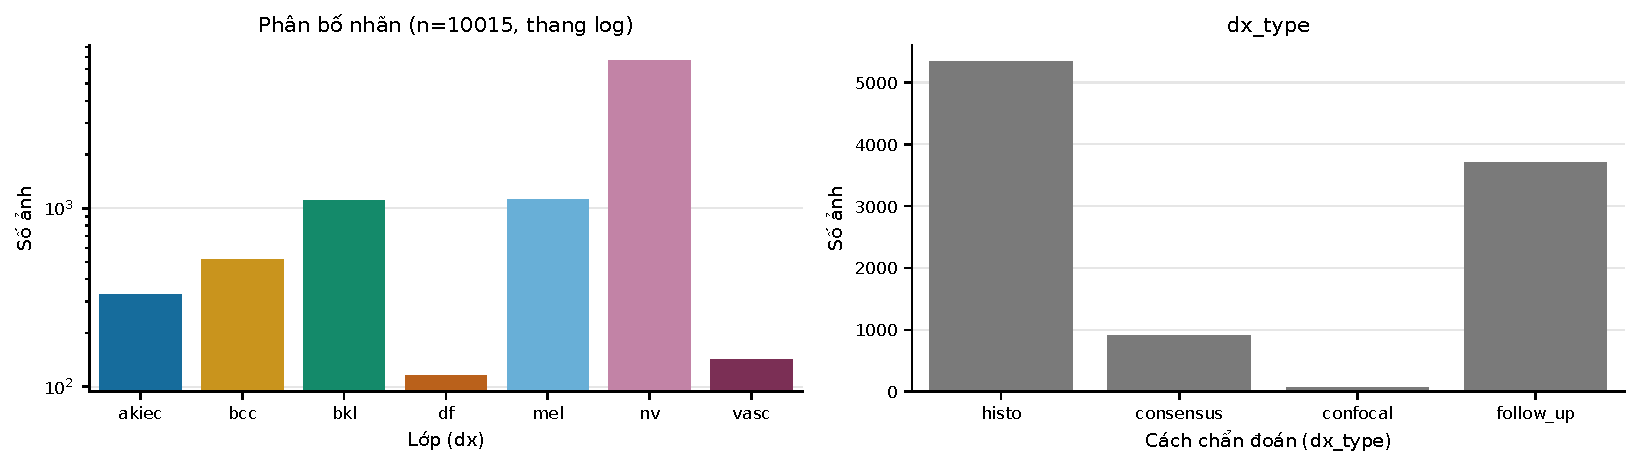
\includegraphics[width=0.98\linewidth]{figures/class_distribution.pdf}
    \caption{Phân bố 7 lớp tổn thương theo thứ tự chuẩn \texttt{sorted(dx)} (trái, thang log; tỉ lệ mất cân bằng $58{,}3\times$) và phương thức xác nhận nhãn \texttt{dx\_type} (phải) trên $n = 10\,015$ ảnh HAM10000.}
    \label{fig:data_wrs}
\end{figure}

\subsection{Phân tích khám phá chất lượng ảnh (EDA -- Trả lời RQ1)}
Thay vì nhận định cảm tính, nhóm xây dựng bộ 7 chỉ số định lượng trên toàn bộ $10\,015$ ảnh (\texttt{src/eda/quality\_metrics.py}). Ngưỡng gắn cờ mặc định tuân theo quy tắc ngoại lai Tukey ($Q_3 + 1{,}5\cdot\text{IQR}$), hoặc ngưỡng tuyệt đối có kiểm tra độ nhạy khi phân phối dồn về 0. Để tránh vi phạm tính độc lập, kiểm định Kruskal--Wallis giữa các lớp \texttt{dx} và nguồn \texttt{dx\_type} được tính trên đúng 1 ảnh/lesion ($n = 7\,470$, hiệu chỉnh Holm) kèm độ lớn hiệu ứng $\varepsilon^2$. Độ nhạy của bộ đo nhiễu được kiểm chứng trước trên 30 ảnh cộng nhiễu tổng hợp đã biết: với nhiễu Gauss $\sigma \in \{0,2,5,10\}$, bộ đo trả về trung vị $1{,}33 / 2{,}39 / 5{,}09 / 9{,}91$; với nhiễu muối--tiêu $p \in \{0{,}1\%, 1\%, 5\%\}$, bộ đo trả về $0{,}099\% / 0{,}98\% / 4{,}97\%$. Do đó, việc chỉ có 1 ảnh thật vượt $0{,}1\%$ pixel xung chứng minh chắc chắn tập ảnh không bị nhiễu muối--tiêu. Chỉ số lông (black-hat $17{\times}17$) cũng khớp thực tế giải phẫu: vùng da đầu (\texttt{scalp}) có $61{,}7\%$ ảnh nhiều lông so với $0\%$ ở lòng bàn tay/chân (\texttt{acral}), và tương quan hạng trước--sau resize $224$ đạt $\rho = 0{,}86$. Ba chỉ số (trắng bạc, nhiễu $\sigma$, viền tối) có $\varepsilon^2$ theo \texttt{dx\_type} lớn gấp 2--4 lần theo \texttt{dx} ($0{,}197$ vs $0{,}088$; $0{,}187$ vs $0{,}044$), củng cố cảnh báo khác biệt nguồn thu nhận (Hình~\ref{fig:eda_sum}). Bảng~\ref{tab:eda_concl} tổng hợp kết luận EDA cùng mức chênh lệch lỗi CNN sau chuẩn hóa thành phần lớp (chi tiết tại mục~\ref{sec:eval}).

\begin{figure}[t]
    \centering
    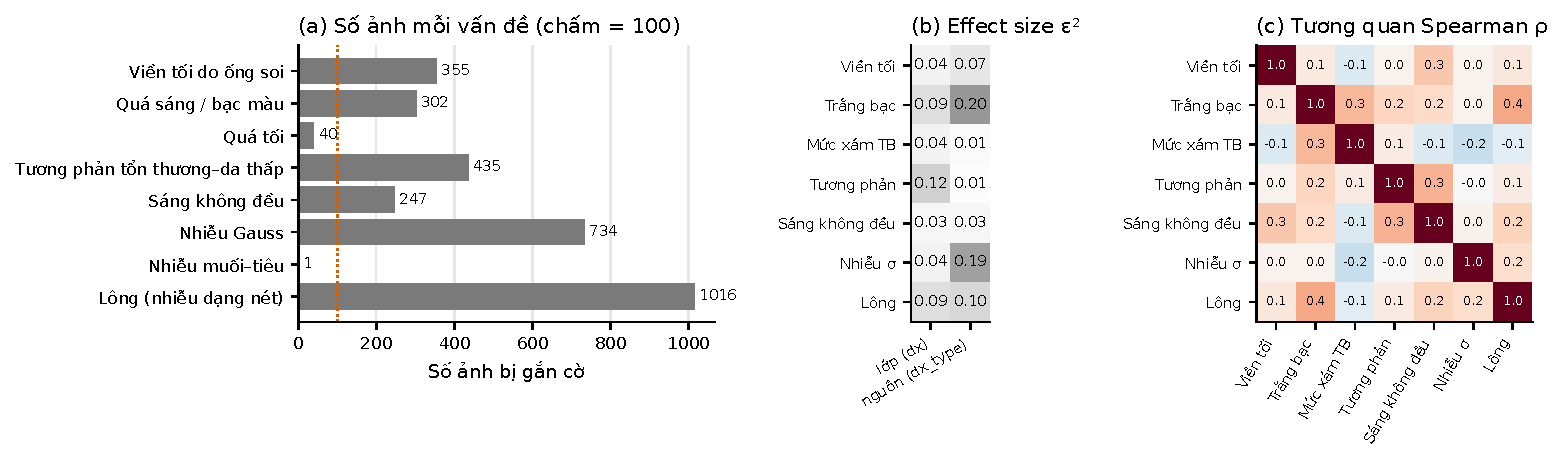
\includegraphics[width=0.98\linewidth]{figures/eda_summary.pdf}
    \caption{Tổng hợp EDA trên $10\,015$ ảnh: (a) quy mô 6 vấn đề tồn tại và 2 vấn đề bác bỏ; (b) so sánh effect size $\varepsilon^2$ theo lớp bệnh \texttt{dx} và nguồn nhãn \texttt{dx\_type}; (c) ma trận tương quan Spearman $|\rho| \le 0{,}40$ khẳng định 7 chỉ số không đo trùng hiện tượng.}
    \label{fig:eda_sum}
\end{figure}

\begin{table*}[!t]
\centering
\caption{Bảng kết luận EDA trên toàn bộ $10\,015$ ảnh và đối chiếu sai số ResNet-18 baseline ngoài mẫu (chuẩn hóa theo thành phần lớp, tập test $n=2\,004$, CI95 bootstrap cụm lesion). Mọi thí nghiệm ở mục 2.5 truy ngược trực tiếp về bảng này.}
\label{tab:eda_concl}
\resizebox{\textwidth}{!}{%
\begin{tabular}{llrrl}
\toprule
\textbf{Vấn đề chất lượng} & \textbf{Định nghĩa chỉ số \& Ngưỡng cờ} & \textbf{Số ảnh (\%)} & \textbf{Lỗi nhóm} & \textbf{Excess lỗi so kỳ vọng lớp [CI95]} \\
\midrule
Lông che phủ & Black-hat $17{\times}17 \ge 20$ ($>5{,}82\%$ FOV) & 1\,016 (10{,}1\%) & $0{,}173$ & $-$0{,}026 [$-$0{,}074; $+0{,}024$] \\
Nhiễu Gauss & $\sigma_{\text{dư}} > 2{{,}}16$ mức xám (vùng phẳng) & 734 (7{,}3\%) & $0{,}065$ & $-$0{,}059 [$-$0{,}093; $-$0{,}023] \\
Tương phản thấp & $\bar{g}_{\text{da}} - \bar{g}_{\text{tổn thương}} < 20$ (Otsu) & 435 (4{,}3\%) & $0{,}251$ & $+0{,}038$ [$-$0{,}031; $+0{,}103$] \\
Viền tối ống soi & Mức xám $\le 20$ nối mép $>1\%$ diện tích & 355 (3{,}5\%) & $0{,}242$ & $+0{,}016$ [$-$0{,}059; $+0{,}094$] \\
Quá sáng (bạc màu) & Pixel $V{\ge}235, S{\le}40 > 10\%$ FOV & 302 (3{,}0\%) & $0{,}271$ & $+0{,}074$ [$-$0{,}020; $+0{,}175$] \\
Sáng không đều & Chênh nền lưới $4{\times}4 > 38$ mức xám & 247 (2{,}5\%) & $0{,}346$ & $+0{,}130$ [$+0{,}024$; $+0{,}230$] \\
Quá tối / Muối--tiêu & $\bar{g}<105{,}6$ / xung $>0{,}1\%$ & 40 / 1 ảnh & -- & Bác bỏ (quá ít mẫu) \\
\bottomrule
\end{tabular}%
}
\end{table*}

\subsection{Làm sạch metadata, Chia tập theo lesion và WRS}
Metadata không có dòng nào thiếu nhãn hay thiếu tệp ảnh; 57 ảnh thiếu \texttt{age} được điền bằng trung vị của riêng tập \texttt{train\_fit} ($50{,}0$ tuổi) kèm cột cờ \texttt{age\_missing} mà không xóa ảnh hợp lệ. Dữ liệu được chia hai tầng bằng \texttt{StratifiedGroupKFold} (nhóm \texttt{lesion\_id}, phân tầng nhãn, \texttt{seed=42}): \texttt{train\_fit} $6\,408$ ảnh ($4\,779$ lesion, $63{,}98\%$), \texttt{val} $1\,603$ ảnh ($1\,196$ lesion, $16{,}01\%$) và \texttt{test} $2\,004$ ảnh ($1\,495$ lesion, $20{,}01\%$), kiểm chứng giao \texttt{lesion\_id} giữa mọi cặp tập bằng $0$. Để xử lý mất cân bằng $58{,}3\times$ trên \texttt{train\_fit}, nhóm dùng \texttt{WeightedRandomSampler} (WRS) với trọng số $w_i = 1/n_{y_i}$ (kỳ vọng mỗi lớp chiếm $14{,}29\%$/epoch) kết hợp \texttt{CrossEntropyLoss} \emph{không} trọng số lớp nhằm tránh bù mất cân bằng hai lần.

\section{Baseline và Khảo sát Kiến trúc CNN}
\textbf{Cấu hình đóng băng.} Mọi thí nghiệm chuẩn hóa ảnh về $224{\times}224$ (PIL bilinear) + ImageNet mean/std, tối ưu bằng AdamW~\cite{loshchilov2019adamw} ($\text{lr}=10^{-4}, \text{wd}=10^{-4}$), batch $32$, $20$ epoch, AMP float16, lật ngang/dọc ngẫu nhiên trên train, chọn checkpoint đạt \texttt{val} macro-F1 cao nhất và đánh giá \texttt{test} đúng 1 lần qua 3 seed ($42, 43, 44$). Bộ phân loại tầm thường luôn đoán \texttt{nv} đạt accuracy $66{,}92\%$ trên test nhưng macro-F1 chỉ $0{,}1145$; do đó \textbf{macro-F1} được dùng làm thước đo chính.

\begin{table}[t]
\centering
\caption{So sánh 3 kiến trúc CNN dưới cùng cấu hình đóng băng (mean $\pm$ std qua 3 seed: 42, 43, 44; $\Delta$ ghép cặp theo seed).}
\label{tab:backbones}
\resizebox{\columnwidth}{!}{%
\begin{tabular}{lrrccc}
\toprule
\textbf{Kiến trúc} & \textbf{Tham số} & \textbf{Val F1} & \textbf{Test F1} & \textbf{Test bAcc} & \textbf{$\Delta$ Test F1} \\
\midrule
ResNet-18 & $11{,}18$M & $0{,}7254 \pm 0{,}0044$ & $\mathbf{0{,}6941 \pm 0{,}0160}$ & $0{,}6777 \pm 0{,}0194$ & Đối chứng \\
EfficientNet-B0 & $4{,}02$M & $0{,}7355 \pm 0{,}0146$ & $\mathbf{0{,}6732 \pm 0{,}0238}$ & $0{,}6478 \pm 0{,}0255$ & $-$0{,}0208 (0+/3-, k.rõ) \\
MobileNetV3-Small & $1{,}53$M & $0{,}6842 \pm 0{,}0306$ & $\mathbf{0{,}6320 \pm 0{,}0125}$ & $0{,}6397 \pm 0{,}0262$ & $-$0{,}0621 (0+/3-, tệ rõ) \\
\bottomrule
\end{tabular}%
}
\end{table}

\begin{figure}[t]
    \centering
    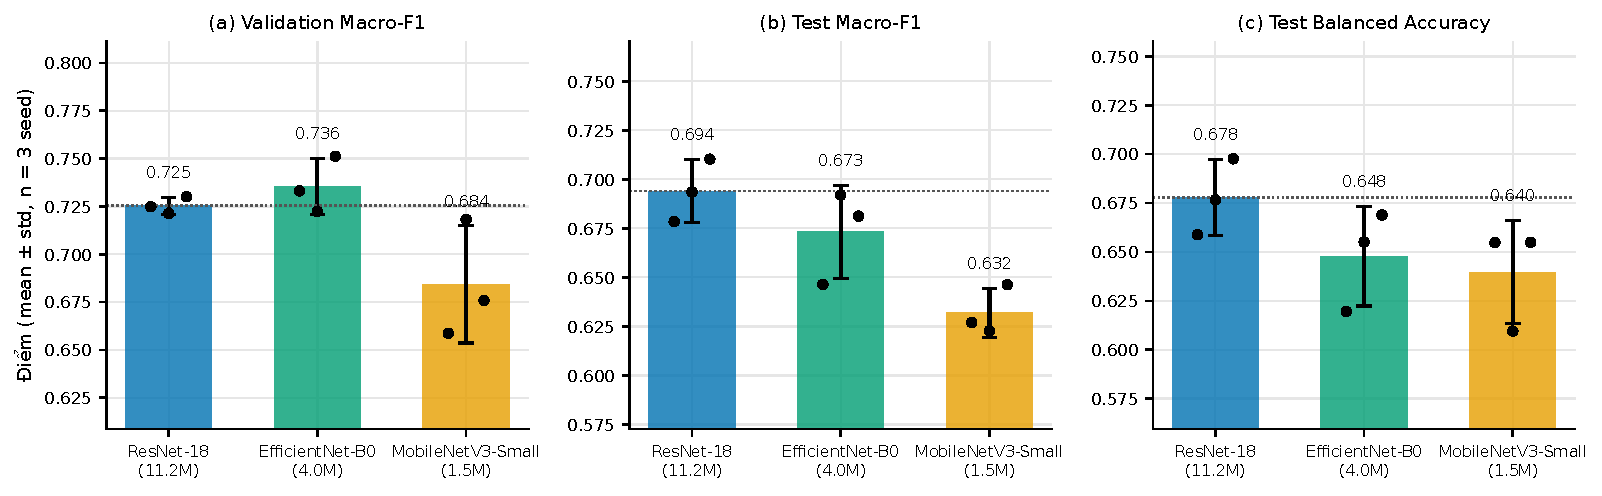
\includegraphics[width=0.98\linewidth]{figures/backbone_comparison.pdf}
    \caption{So sánh hiệu năng 3 kiến trúc CNN đại diện (cột = trung bình, vạch = $\pm 1$ std, chấm = từng seed 42/43/44).}
    \label{fig:backbones}
\end{figure}

Bảng~\ref{tab:backbones} và Hình~\ref{fig:backbones} trình bày kết quả khảo sát 3 họ kiến trúc (với \texttt{EfficientNet-B0} và \texttt{MobileNetV3-Small} dùng tích lũy gradient \texttt{micro\_batch}$=16$ để tiết kiệm VRAM khối MBConv). Theo nguyên tắc chọn trên \texttt{val} (không dùng \texttt{test}), dù \texttt{EfficientNet-B0} có trung bình \texttt{val} F1 nhỉnh nhẹ ($0{,}7355 \pm 0{,}0146$), \texttt{ResNet-18} có độ lệch chuẩn giữa các seed trên \texttt{val} thấp hơn gấp $3{,}3$ lần ($0{,}0044$), cấu trúc khối dư tường minh và lưới đặc trưng \texttt{layer4} ($7{\times}7$) thuận lợi cho Grad-CAM nên được khóa làm mô hình cơ sở xuyên suốt 16 thí nghiệm mục~\ref{sec:ablation}. Trên \texttt{test}, \texttt{ResNet-18} đạt macro-F1 $0{,}6941 \pm 0{,}0160$ (bAcc $0{,}6777 \pm 0{,}0194$, Acc $0{,}8315 \pm 0{,}0032$), vượt rõ \texttt{MobileNetV3-Small} và không khác biệt thống kê với \texttt{EfficientNet-B0} (CI95 $[$-$0{,}0552; $+0{,}0164$]$ phủ $0$).

\section{Thực nghiệm Tiền xử lý Ảnh có Kiểm soát}
\label{sec:ablation}
\textbf{Quy tắc kết luận đặt trước (2.5.0).} Mọi phép xử lý áp ở độ phân giải gốc $600{\times}450$ trước resize $224$, đồng nhất cho cả 3 tập. Một cấu hình chỉ được kết luận là ``tốt hơn rõ'' hoặc ``tệ hơn rõ'' khi thỏa cả 3 điều kiện: (1) $|\Delta\text{ trung bình}| > \text{std}_{\text{baseline}}$ trên cùng split; (2) khoảng tin cậy $95\%$ bootstrap theo cụm \texttt{lesion\_id} ($1\,000$ lần) không chứa $0$; và (3) cả $3/3$ seed cùng dấu. \emph{Lưu ý thống kê:} phép bootstrap lấy mẫu lại cụm \texttt{lesion\_id} trên 3 checkpoint cố định nên đo bất định mẫu đánh giá (chưa gộp phương sai huấn luyện lại giữa các seed khi 16 cấu hình cùng so với một bộ 3 seed baseline có test F1 cao $0{,}6941 \pm 0{,}0160$); do đó mọi quyết định chọn pipeline ở mục~\ref{sec:eval} chỉ căn cứ trên \texttt{val} kết hợp kiểm định nhóm con DiD.

\subsection{Nhiễu Gauss và Tương phản thấp (Chương 3 \& 4)}
Với nhiễu Gauss, nhóm đối chiếu lọc Gauss $3{\times}3$ (nhân $\frac{1}{16}[1\,2\,1;2\,4\,2;1\,2\,1]$), trung vị $3{\times}3$ và trung vị $5{\times}5$. Đo trực tiếp trên $463$ ảnh cờ nhiễu thuộc \texttt{train\_fit} cho thấy resize $600{\rightarrow}224$ vốn đã hạ $\sigma$ Immerkaer~\cite{immerkaer1996fast} từ $1{,}58$ xuống $0{,}86$; lọc \texttt{median5} hạ tiếp xuống $0{,}385$ nhưng làm mất $75\%$ phương sai Laplacian vùng tổn thương. Với tương phản thấp, nhóm biến đổi kênh độ sáng $L^*$ của không gian CIE $L^*a^*b^*$ để hạn chế bóp méo sắc độ $a^*,b^*$: giãn phân vị $[P_1, P_{99}]$ (\texttt{stretch\_L\_1\_99}), cân bằng lược đồ toàn cục (\texttt{hist\_eq\_L}) và CLAHE cục bộ \texttt{clahe\_L\_c2\_t8} (clip $2{,}0$, lưới $8{\times}8$). Kiểm tra trực quan từng khung trên mẫu ngẫu nhiên 24 ảnh cờ tương phản thấp (\texttt{seed=42}) ghi nhận mask Otsu thô chỉ bao đúng $8/24$ ảnh, đúng một phần $5/24$ và bao sai $11/24$ ảnh (thường bắt bóng tối rìa ảnh). Trên CNN (Bảng~\ref{tab:all16}), \texttt{hist\_eq\_L} và \texttt{stretch\_L\_1\_99} đều \textbf{tệ hơn rõ} trên cả \texttt{val} lẫn \texttt{test} ($0+/3-$, CI95 tách rời 0) vì làm biến thiên mạnh độ chói ($\Delta E_{76}$ từ $14$ đến $22$, chủ yếu do $\Delta L^*$ xóa thông tin độ tối tuyệt đối kèm trượt sắc độ $\Delta ab \approx 1{,}5$ khi cắt biên sRGB) và nhân nhiễu lên $3{,}5\text{--}5{,}5$ lần trên $95{,}7\%$ ảnh thường; ngược lại \texttt{median3} và \texttt{clahe\_L\_c2\_t8} giữ trung tính.

\subsection{Lông, Viền tối, Quá sáng và Sáng lệch: Đại trà vs Có điều kiện}
Vì mỗi lỗi chỉ chiếm $2{,}5\%\text{--}10{,}1\%$ dữ liệu, nhóm thiết kế đối chứng giữa \textbf{bản đại trà} và \textbf{bản có điều kiện} (kích hoạt theo ngưỡng cờ không giám sát của EDA -- kiểm tra lại trên riêng \texttt{train\_fit} cho ngưỡng \texttt{illum\_range} khớp tuyệt đối $38{,}00$ và \texttt{hair\_frac} lệch chỉ $0{,}11\%$ FOV; hằng số mục tiêu \texttt{L\_TARGET}$=66{,}61$ chỉ tính trên \texttt{train\_fit}):
\begin{itemize}
    \item \textbf{Lông (Ch.7 + Ch.3):} Black-hat elip $17{\times}17 \ge 20$ + giãn $3{\times}3$ + Telea inpainting bán kính 5 px~\cite{lee1997dullrazor,telea2004inpainting} (\texttt{hair\_bh17} và \texttt{hair\_bh17\_cond}).
    \item \textbf{Viền tối (Ch.3 + Ch.7):} Tô vùng đen nối mép bằng trung vị dải da 25 px + làm mềm biên Gauss $21{\times}21$ (\texttt{vig\_fill}, giữ nguyên tỉ lệ tổn thương) đối chiếu cắt khung đồng tâm 4:3 (\texttt{vig\_crop}).
    \item \textbf{Quá sáng \& Sáng lệch (Ch.3 + Ch.4):} Biến đổi lũy thừa $s=r^\gamma$ trên $L^*$ (\texttt{gamma\_L\_1.5} vs \texttt{gamma\_L\_auto} tự chọn $\gamma \in [1;3]$) và chia trường sáng nền Gauss chuẩn hóa $\sigma=60$ px ngoài vùng tổn thương (\texttt{flat\_L\_s60} vs \texttt{flat\_L\_s60\_cond}).
\end{itemize}

\begin{table*}[!t]
\centering
\caption{Kết quả tổng hợp thực nghiệm Ablation 16 cấu hình tiền xử lý trên ResNet-18 (3 seed: 42, 43, 44; cùng một phần cứng NVIDIA L40S). Không cấu hình nào đạt ``tốt hơn rõ'' trên validation; 2 phép toàn cục giảm mạnh hiệu năng.}
\label{tab:all16}
\resizebox{\textwidth}{!}{%
\begin{tabular}{llccccl}
\toprule
\textbf{Nhóm} & \textbf{Cấu hình} & \textbf{Val Macro-F1} & \textbf{$\Delta$ Val (dấu)} & \textbf{Test Macro-F1} & \textbf{$\Delta$ Test [CI95 bootstrap]} & \textbf{Kết luận (Test)} \\
\midrule
Đối chứng & \texttt{baseline} & $0{,}7254 \pm 0{,}0044$ & -- & $0{,}6941 \pm 0{,}0160$ & -- & Đối chứng \\
Nhiễu & \texttt{gauss3} & $0{,}7238 \pm 0{,}0141$ & $-$0{,}0016 (1+/2-) & $0{,}6422 \pm 0{,}0180$ & $-$0{,}0518 [$-$0{,}0762; $-$0{,}0280] & \textbf{Tệ hơn rõ} \\
Nhiễu & \texttt{median3} & $0{,}7294 \pm 0{,}0088$ & $+0{,}0040$ (2+/1-) & $0{,}6833 \pm 0{,}0032$ & $-$0{,}0107 [$-$0{,}0364; $+0{,}0164$] & Không rõ \\
Nhiễu & \texttt{median5} & $0{,}7196 \pm 0{,}0194$ & $-$0{,}0059 (1+/2-) & $0{,}6720 \pm 0{,}0030$ & $-$0{,}0221 [$-$0{,}0553; $+0{,}0089$] & Không rõ \\
T.phản & \texttt{stretch\_L\_1\_99} & $0{,}6920 \pm 0{,}0133$ & $-$0{,}0334 (0+/3-) & $0{,}6154 \pm 0{,}0172$ & $-$0{,}0786 [$-$0{,}1149; $-$0{,}0442] & \textbf{Tệ hơn rõ} \\
T.phản & \texttt{hist\_eq\_L} & $0{,}6472 \pm 0{,}0061$ & $-$0{,}0782 (0+/3-) & $0{,}5834 \pm 0{,}0217$ & $-$0{,}1106 [$-$0{,}1508; $-$0{,}0698] & \textbf{Tệ hơn rõ} \\
T.phản & \texttt{clahe\_L\_c2\_t8} & $0{,}7261 \pm 0{,}0205$ & $+0{,}0007$ (1+/2-) & $0{,}6706 \pm 0{,}0071$ & $-$0{,}0235 [$-$0{,}0524; $+0{,}0088$] & Không rõ \\
Lông & \texttt{hair\_bh17} & $0{,}7044 \pm 0{,}0130$ & $-$0{,}0210 (0+/3-) & $0{,}6577 \pm 0{,}0104$ & $-$0{,}0363 [$-$0{,}0678; $-$0{,}0038] & \textbf{Tệ hơn rõ} \\
Lông & \texttt{hair\_bh17\_cond} & $0{,}7213 \pm 0{,}0109$ & $-$0{,}0041 (1+/2-) & $0{,}6539 \pm 0{,}0121$ & $-$0{,}0402 [$-$0{,}0689; $-$0{,}0080] & \textbf{Tệ hơn rõ} \\
Viền & \texttt{vig\_fill} & $0{,}7130 \pm 0{,}0113$ & $-$0{,}0124 (1+/2-) & $0{,}6978 \pm 0{,}0161$ & $+0{,}0038$ [$-$0{,}0212; $+0{,}0291$] & Không rõ \\
Viền & \texttt{vig\_crop} & $0{,}7240 \pm 0{,}0057$ & $-$0{,}0014 (0+/3-) & $0{,}6578 \pm 0{,}0171$ & $-$0{,}0363 [$-$0{,}0679; $-$0{,}0083] & \textbf{Tệ hơn rõ} \\
Q.sáng & \texttt{gamma\_L\_1.5} & $0{,}7161 \pm 0{,}0081$ & $-$0{,}0093 (0+/3-) & $0{,}6930 \pm 0{,}0203$ & $-$0{,}0010 [$-$0{,}0249; $+0{,}0198$] & Không rõ \\
Q.sáng & \texttt{gamma\_L\_auto} & $0{,}7215 \pm 0{,}0042$ & $-$0{,}0039 (0+/3-) & $0{,}6786 \pm 0{,}0005$ & $-$0{,}0155 [$-$0{,}0466; $+0{,}0113$] & Không rõ \\
S.lệch & \texttt{flat\_L\_s60} & $0{,}7231 \pm 0{,}0081$ & $-$0{,}0023 (1+/2-) & $0{,}6686 \pm 0{,}0320$ & $-$0{,}0254 [$-$0{,}0503; $+0{,}0008$] & Không rõ \\
S.lệch & \texttt{flat\_L\_s60\_cond} & $0{,}7247 \pm 0{,}0019$ & $-$0{,}0007 (2+/1-) & $0{,}6789 \pm 0{,}0035$ & $-$0{,}0151 [$-$0{,}0450; $+0{,}0108$] & Không rõ \\
Kết hợp & \texttt{median3+clahe\_L\_c2\_t8} & $0{,}7209 \pm 0{,}0068$ & $-$0{,}0045 (1+/2-) & $0{,}6719 \pm 0{,}0279$ & $-$0{,}0222 [$-$0{,}0459; $+0{,}0011$] & Không rõ \\
Kết hợp & \texttt{vig\_fill+flat\_L\_s60\_cond} & $0{,}7304 \pm 0{,}0147$ & $+0{,}0050$ (2+/1-) & $0{,}6635 \pm 0{,}0146$ & $-$0{,}0305 [$-$0{,}0576; $-$0{,}0019] & \textbf{Tệ hơn rõ} \\
\bottomrule
\end{tabular}%
}
\end{table*}

\begin{figure*}[!t]
    \centering
    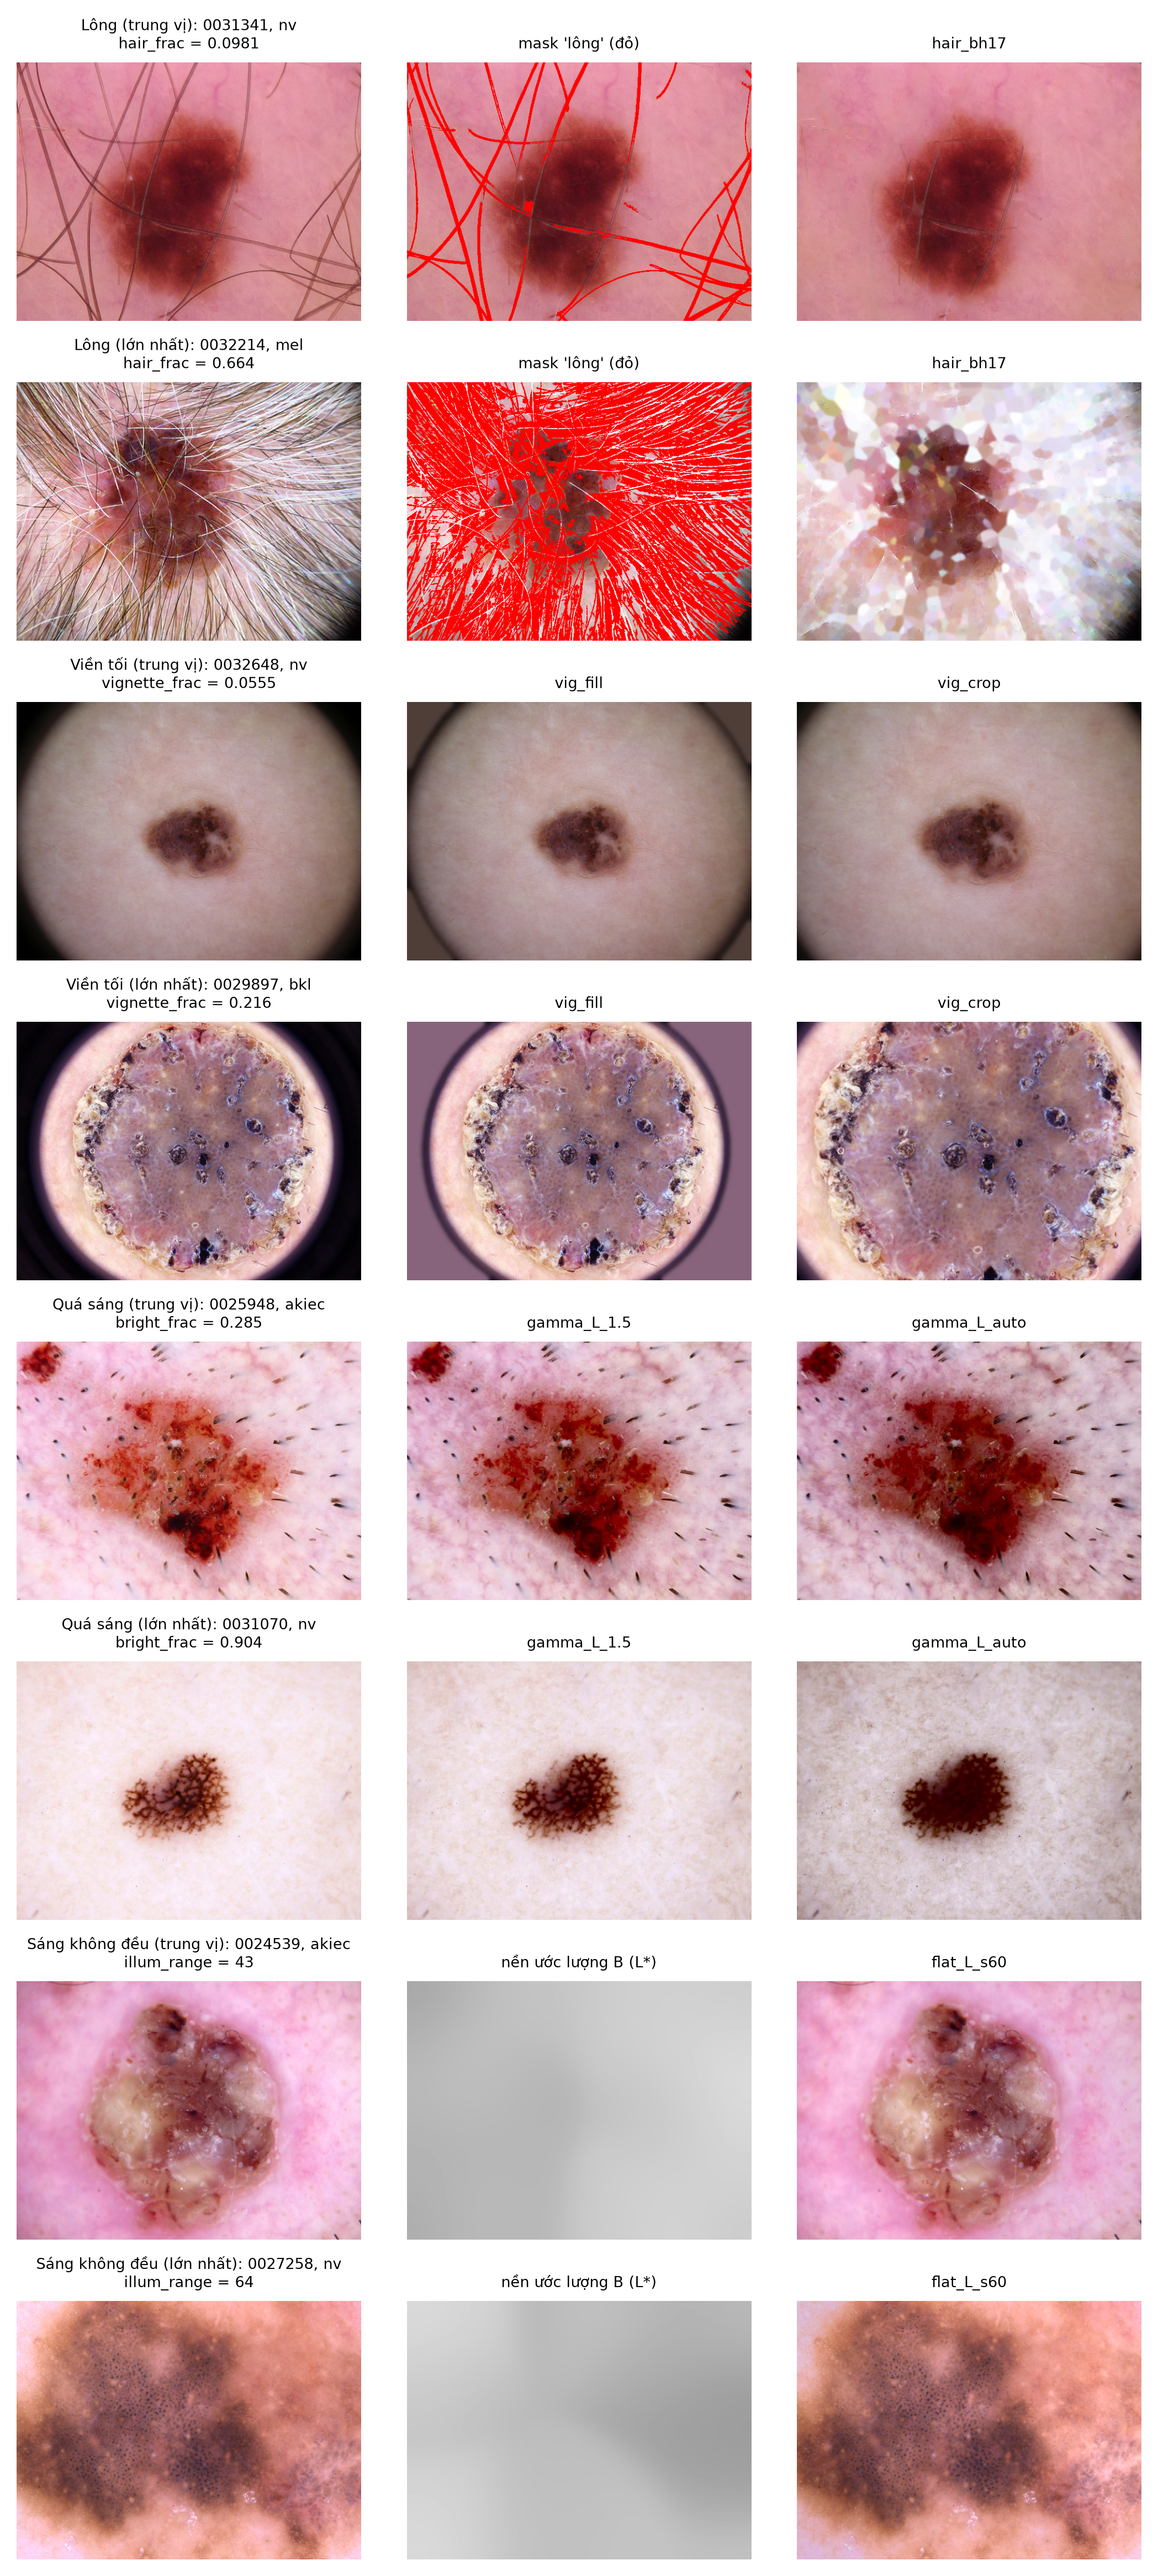
\includegraphics[height=0.56\textheight,keepaspectratio]{figures/artifacts_before_after.png}
    \caption{Đối chiếu trực quan ảnh gốc, mask phát hiện và ảnh sau xử lý của 4 phép biến đổi có điều kiện (xóa lông \texttt{hair\_bh17\_cond}, lấp viền tối \texttt{vig\_fill}, chỉnh sáng tự động \texttt{gamma\_L\_auto} và cân bằng trường sáng \texttt{flat\_L\_s60\_cond}) trên các ca bị cờ EDA.}
    \label{fig:artifacts_ba}
\end{figure*}

\begin{figure}[t]
    \centering
    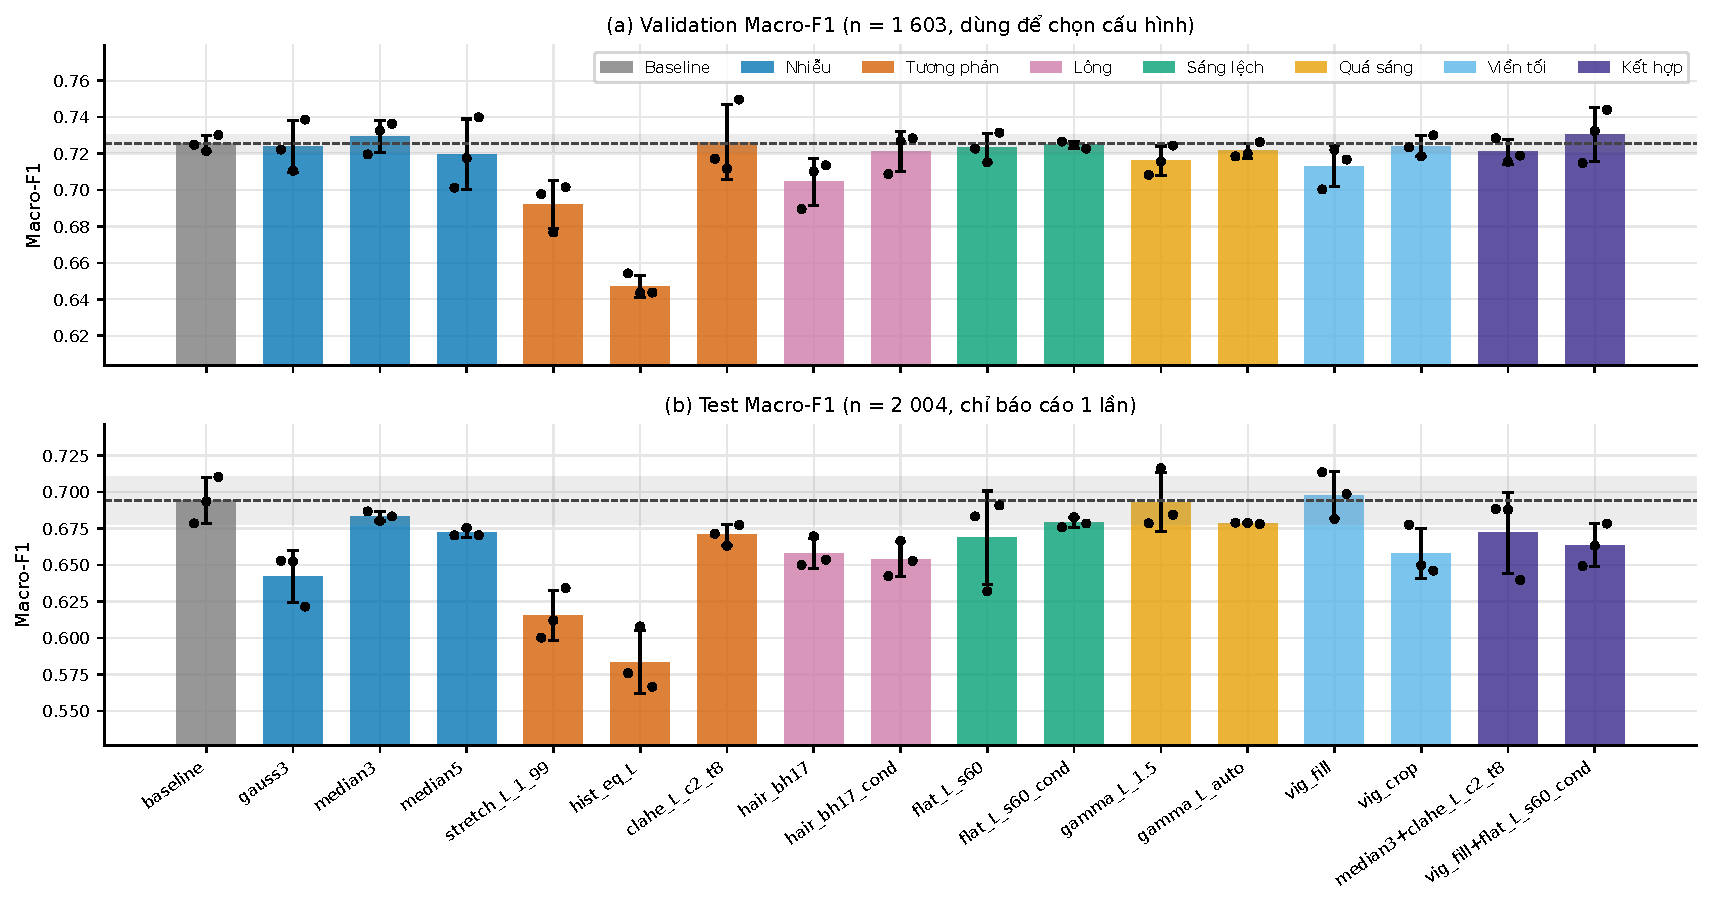
\includegraphics[width=0.98\linewidth]{figures/all16_macro_f1.pdf}
    \caption{Macro-F1 trên Validation và Test của baseline cùng 16 cấu hình tiền xử lý (dải xám ngang = $\pm 1$ std của baseline; chấm đen = từng seed 42, 43, 44).}
    \label{fig:all16}
\end{figure}

Bảng~\ref{tab:all16}, Hình~\ref{fig:artifacts_ba} và Hình~\ref{fig:all16} cho thấy cả 8 cấu hình thuộc nhóm này và 2 cấu hình kết hợp đều không vượt chuẩn cải thiện rõ trên \texttt{val}. Phân tích sai số kép (DiD) trên nhóm ảnh bị cờ có khoảng tin cậy 95\% phủ 0 ở 7/8 cấu hình, ngoại trừ \texttt{gamma\_L\_auto} làm giảm mạnh độ chính xác ngay trên 69 ảnh quá sáng tập test ($0{,}729 \rightarrow 0{,}507$, $\text{DiD} = $-$0{,}209$ $[$-$0{,}302; $-$0{,}116]$) do lệch phân phối có điều kiện trên $3\%$ dữ liệu và kéo vùng lóa mất sắc độ ($a^*,b^*\approx 0$) thành mảng xám nhân tạo. Các bản có điều kiện giữ nguyên $100\%$ ảnh đối chứng (các nhãn ``tệ hơn rõ'' ở \texttt{vig\_crop} hay \texttt{vig\_fill+flat\_L\_s60\_cond} dù nhóm cờ tăng $+0{,}004$ đến $+0{,}036$ xuất phát từ nhiễu huấn luyện lại trên các lớp nhỏ không bị cờ), trong khi \texttt{hair\_bh17} đại trà sửa nhầm $92\%$ ảnh không lông và giảm điểm cả 3/3 seed.

\subsection{Phân tích sâu 4 tầng tác động (Mục 2.5c -- Trả lời RQ3)}
Để giải thích vì sao cải thiện chỉ số ảnh không chuyển hóa thành tăng macro-F1 trên tập ảnh gốc, nhóm định lượng tiếp trên 4 tầng (Hình~\ref{fig:impact4}):
\begin{enumerate}
    \item \textbf{Tầng A (Mức ảnh trên \texttt{train\_fit}):} Các phép xử lý xóa $91{,}8\%\text{--}100\%$ cờ viền, lông, quá sáng, sáng lệch. Tuy nhiên, kiểm định trên toàn bộ \texttt{train\_fit} phát hiện \texttt{hair\_bh17} inpaint trung vị $\mathbf{8.9\%}$ diện tích vùng tổn thương của \texttt{mel}, cao gấp hơn 3 lần so với $\mathbf{2.5\%}$ ở \texttt{nv} (Mann--Whitney 1 ảnh/lesion $p = 7.4e-46$, Cliff's $\delta = 0{,}436$). Ngoài ra, trên ca lông bạc/trắng dày (\texttt{ISIC\_0032214}), black-hat bắt nhầm nền da tối giữa các sợi lông sáng làm nhòe mảng tổn thương.
    \item \textbf{Tầng B (Đổi nhãn dự đoán so với mức nền):} Giữa 2 seed khác nhau của chính baseline vốn đã có $15{,}3\%$ ảnh test đổi nhãn dự đoán ($15{,}9\%$ trên \texttt{val}). Tỉ lệ đổi nhãn toàn tập của \texttt{vig\_fill} ($-0{,}67\%$) và \texttt{flat\_L\_s60\_cond} ($-0{,}12\%$, $p_{\text{Holm}}=1{,}00$) nằm đúng mức nền tự nhiên này; riêng \texttt{gamma\_L\_auto} sát mức nền trên ảnh không cờ ($+0{,}71\%$) nhưng vọt $+20{,}53\%$ lật nhãn trên nhóm quá sáng ($p_{\text{Holm}}=0{,}005$), còn \texttt{hair\_bh17}/\texttt{hair\_bh17\_cond} vượt nền rõ ($+2{,}35\%/+2{,}45\%$).
    \item \textbf{Tầng C (Stress Test suy giảm tổng hợp):} Khi áp 6 loại suy giảm $\times$ 3 mức độ lên tập đánh giá (Bảng~\ref{tab:stress}), tiền xử lý khôi phục mạnh ở mức suy giảm nặng ngay trên nhánh \texttt{test\_only}: \texttt{hair\_bh17\_cond} tăng $+0{,}4623$ macro-F1 (lông dày), \texttt{clahe\_L\_c2\_t8} tăng $+0{,}1943$ (nén tương phản $0{,}3\times$) và \texttt{vig\_fill} tăng $+0{,}1020$ (viền lớn), đều đạt ``tốt hơn rõ'' ($3+/0-$). Đáng chú ý, ở \texttt{low\_contrast}, \texttt{clahe\_L\_c2\_t8} giúp nhánh \texttt{test\_only} tăng $+0{,}1943$ nhưng nhánh \texttt{retrain} chỉ đạt $-0{,}0073$ vì CLAHE đưa ảnh bị nén $0{,}3\times$ trở về sát phân phối gốc mà \texttt{baseline} quen thuộc, trong khi mô hình \texttt{retrain} lại kỳ vọng độ tương phản cao hơn nữa. Với \texttt{overexpose} mức 3, \texttt{gamma\_L\_auto} không khôi phục được thông tin bão hòa 255 ($-0{,}0005$).
    \item \textbf{Tầng D (Grad-CAM \texttt{layer4}):} Xóa viền tối và xóa lông giúp giảm tỉ lệ năng lượng Grad-CAM rơi vào góc viền/sợi lông và giữ tương đồng bản đồ nhiệt Pearson $r$ ổn định quanh mức nền giữa các seed, song bản thân baseline vốn đã tập trung phần lớn năng lượng vào vùng tổn thương trung tâm.
\end{enumerate}

\begin{table*}[!t]
\centering
\caption{Stress Test tầng C (Mức suy giảm nặng nhất -- Mức 3, tập test): $\Delta$ Macro-F1 so với baseline không xử lý trên cùng ảnh suy giảm.}
\label{tab:stress}
\footnotesize
\begin{tabular}{llccc}
\toprule
\textbf{Suy giảm (Mức 3)} & \textbf{Phép xử lý} & \textbf{Tỉ lệ kích hoạt} & \textbf{Nhánh test\_only} & \textbf{Nhánh retrain} \\
\midrule
\texttt{noise} (40.0) & \texttt{median3} & 100\% & $+0{,}0474$ (không khác biệt rõ) & $+0{,}0018$ (không khác biệt rõ) \\
\texttt{low\_contrast} (0.3) & \texttt{clahe\_L\_c2\_t8} & 100\% & $+0{,}1943$ (tốt hơn rõ) & $-$0{,}0073 (không khác biệt rõ) \\
\texttt{overexpose} (1.7) & \texttt{gamma\_L\_auto} & 53\% & $-$0{,}0005 (không khác biệt rõ) & $-$0{,}0188 (không khác biệt rõ) \\
\texttt{uneven} (0.7) & \texttt{flat\_L\_s60\_cond} & 27\% & $-$0{,}0082 (không khác biệt rõ) & $-$0{,}0210 (không khác biệt rõ) \\
\texttt{uneven} (0.7) & \texttt{flat\_L\_s60} & 100\% & $-$0{,}0396 (tệ hơn rõ) & $-$0{,}0729 (tệ hơn rõ) \\
\texttt{vignette} (0.7) & \texttt{vig\_fill} & 100\% & $+0{,}1020$ (tốt hơn rõ) & $+0{,}0899$ (tốt hơn rõ) \\
\texttt{hair} (60.0) & \texttt{hair\_bh17\_cond} & 100\% & $+0{,}4623$ (tốt hơn rõ) & $+0{,}4322$ (tốt hơn rõ) \\
\texttt{hair} (60.0) & \texttt{hair\_bh17} & 100\% & $+0{,}4623$ (tốt hơn rõ) & $+0{,}4307$ (tốt hơn rõ) \\
\bottomrule
\end{tabular}
\end{table*}

\begin{figure}[t]
    \centering
    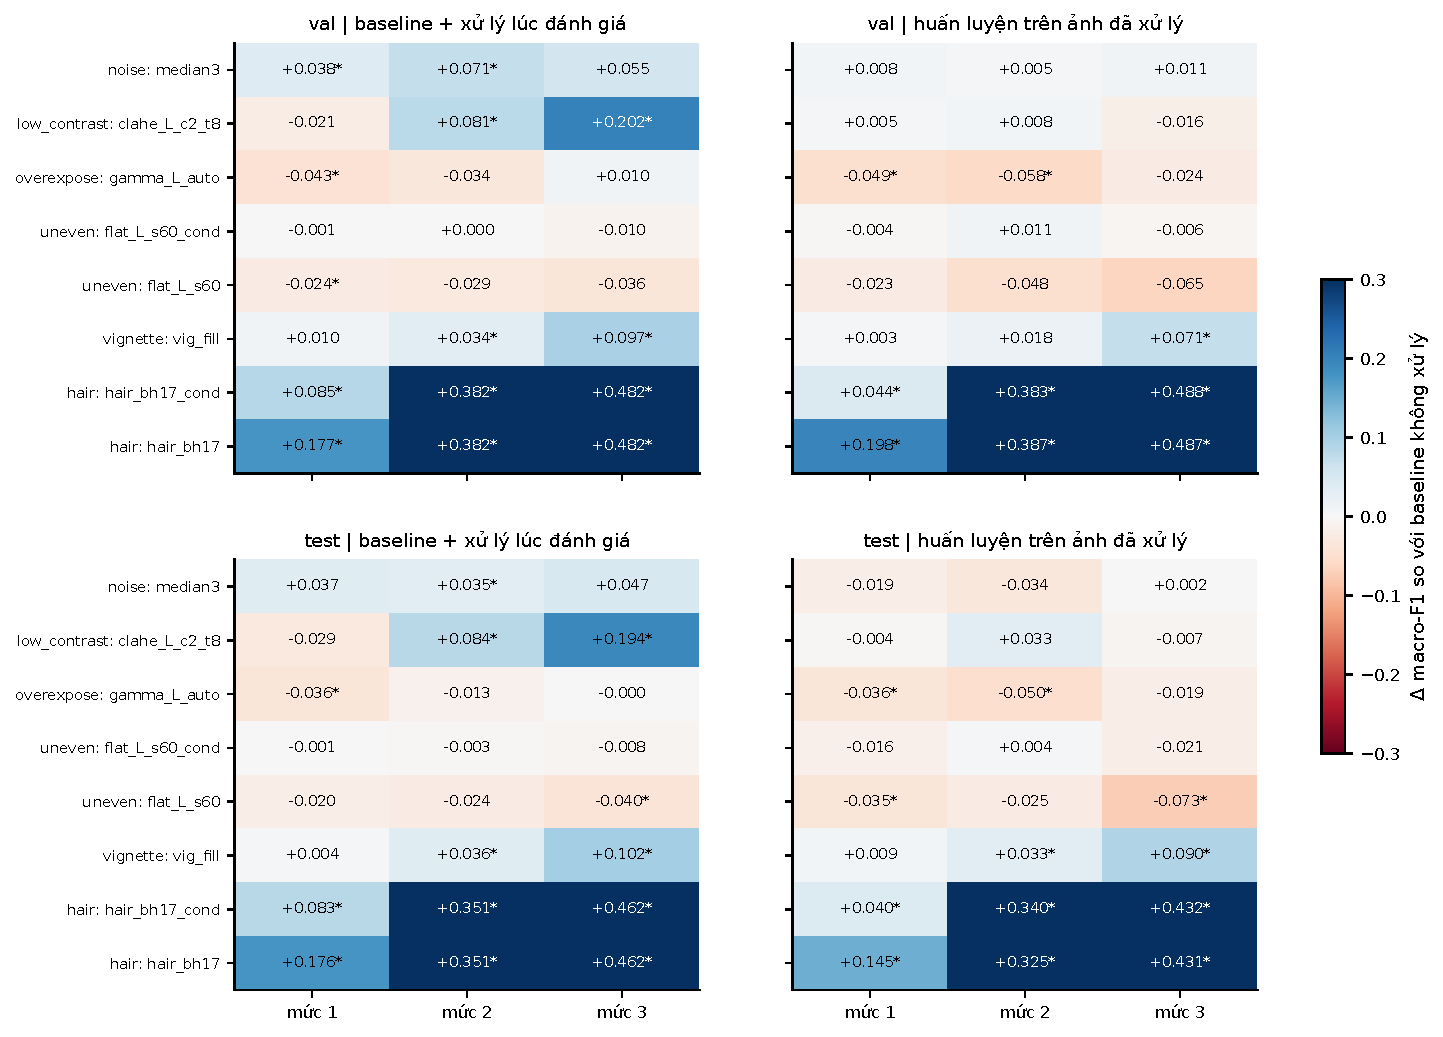
\includegraphics[width=0.98\linewidth]{figures/impact_c2_stress.pdf}
    \caption{Bản đồ nhiệt $\Delta$ Macro-F1 trong Stress Test 18 điều kiện suy giảm tổng hợp (dấu $*$ đánh dấu khác biệt rõ theo quy tắc 2.5.0).}
    \label{fig:impact4}
\end{figure}

\section{Pipeline Đề xuất, Đánh giá Lỗi \& Demo}
\label{sec:eval}
\subsection{Kiến trúc Pipeline hai nhánh và Mô hình cuối (2.6--2.7)}
Áp dụng quy tắc chọn 3 điều kiện trên \texttt{val}, không bước biến đổi pixel nào được đưa vào nhánh phân loại tự động (trả lời \textbf{RQ4}: ghép nối \texttt{median3+clahe\_L\_c2\_t8} hay \texttt{vig\_fill+flat\_L\_s60\_cond} cũng không vượt thành phần đơn lẻ). Pipeline đề xuất gồm \textbf{hai nhánh song song}:
\begin{itemize}
    \item \textbf{Nhánh (A) Kiểm tra chất lượng (QC):} chạy bộ đo 6 chỉ số Chương 3--7 trên ảnh $600{\times}450$ để gắn cờ cảnh báo cho người dùng (đặc biệt cảnh báo khi gặp \emph{sáng không đều} và \emph{quá sáng}), đồng thời cho phép bật tường minh các bước có điều kiện (\texttt{vig\_fill}, \texttt{flat\_L\_s60\_cond}) để quan sát đối chiếu.
    \item \textbf{Nhánh (B) Phân loại chính:} đưa ảnh RGB gốc qua \texttt{Resize 224} $\rightarrow$ \texttt{Normalize ImageNet} $\rightarrow$ \texttt{ResNet-18} (giữ nguyên cấu hình đóng băng mục 2.4). Bản demo nạp checkpoint \texttt{baseline\_seed42.pt} (hạt giống mặc định đặt trước, hội tụ tại epoch 11, test macro-F1 $0{,}6784$).
\end{itemize}

\subsection{Phân tích lỗi chuyên sâu và Demo Streamlit (2.8)}
\begin{table}[t]
\centering
\caption{Hiệu năng theo từng lớp trên tập test ($n=2\,004$, 3 seed) và tỉ lệ ảnh khó bị đoán sai nhất quán ở cả 3 seed.}
\label{tab:perclass}
\resizebox{\columnwidth}{!}{%
\begin{tabular}{lrrccr}
\toprule
\textbf{Lớp} & \textbf{$n$ test} & \textbf{Precision} & \textbf{Recall} & \textbf{F1-score} & \textbf{Sai cả 3 seed} \\
\midrule
\texttt{akiec} & 66 & $0{,}611$ & $0{,}510 \pm 0{,}162$ & $0{,}551 \pm 0{,}122$ & 16 (24{,}2\%) \\
\texttt{bcc} & 103 & $0{,}690$ & $0{,}828 \pm 0{,}072$ & $0{,}751 \pm 0{,}034$ & 5 (4{,}9\%) \\
\texttt{bkl} & 220 & $0{,}667$ & $0{,}729 \pm 0{,}051$ & $0{,}695 \pm 0{,}012$ & 28 (12{,}7\%) \\
\texttt{df} & 23 & $0{,}870$ & $0{,}522 \pm 0{,}075$ & $0{,}647 \pm 0{,}053$ & 8 (34{,}8\%) \\
\texttt{mel} & 222 & $0{,}588$ & $0{,}518 \pm 0{,}090$ & $0{,}546 \pm 0{,}036$ & 61 (27{,}5\%) \\
\texttt{nv} & 1341 & $0{,}921$ & $0{,}924 \pm 0{,}009$ & $0{,}922 \pm 0{,}002$ & 27 (2{,}0\%) \\
\texttt{vasc} & 29 & $0{,}786$ & $0{,}713 \pm 0{,}080$ & $0{,}747 \pm 0{,}075$ & 5 (17{,}2\%) \\
\bottomrule
\end{tabular}%
}
\end{table}

\begin{figure}[t]
    \centering
    \begin{subfigure}[b]{0.49\linewidth}
        \centering
        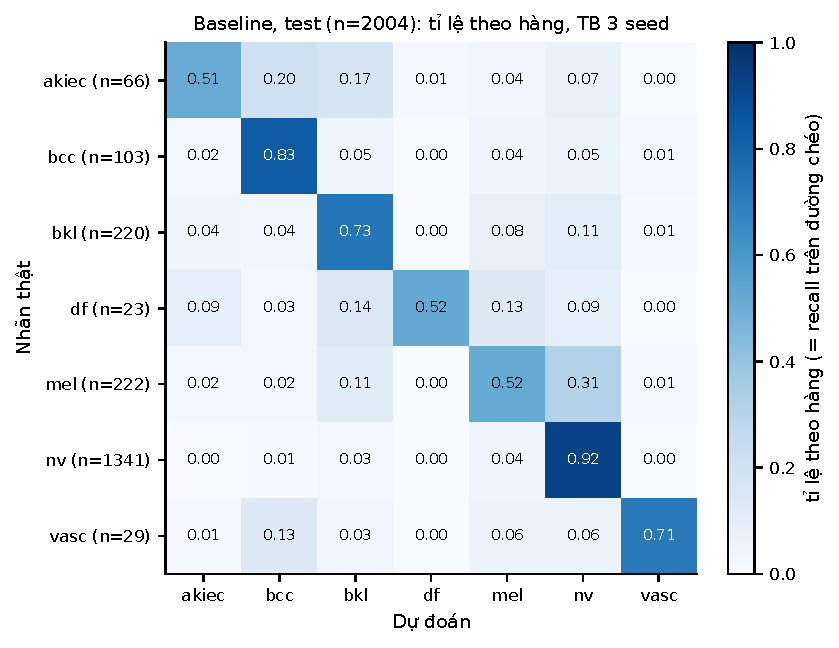
\includegraphics[width=\linewidth]{figures/confusion_test.pdf}
        \caption{Confusion matrix test}
    \end{subfigure}
    \hfill
    \begin{subfigure}[b]{0.49\linewidth}
        \centering
        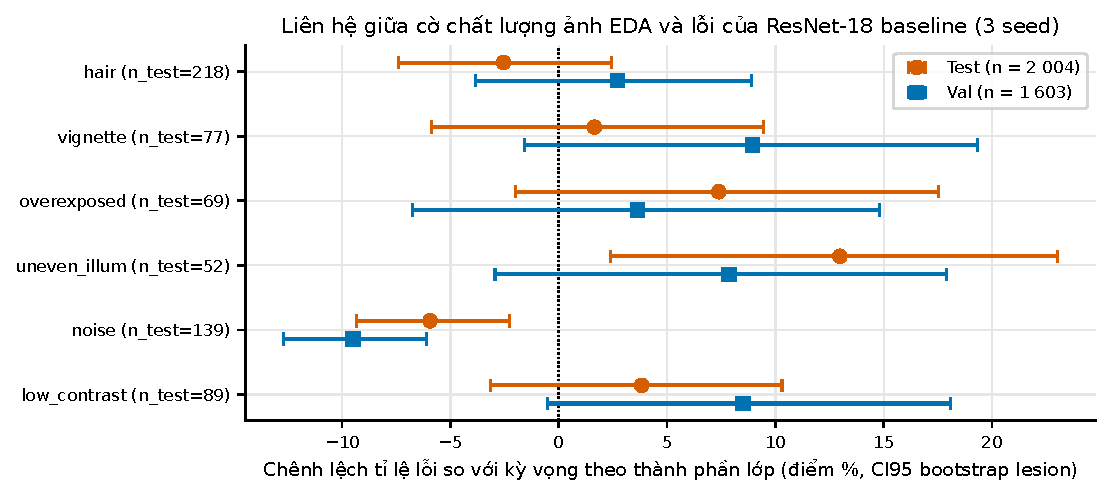
\includegraphics[width=\linewidth]{figures/eda_cnn_link.pdf}
        \caption{Excess lỗi theo cờ EDA}
    \end{subfigure}
    \caption{(a) Ma trận nhầm lẫn chuẩn hóa theo hàng của mô hình cuối (TB 3 seed); (b) Chênh lệch lỗi của nhóm cờ EDA sau khi chuẩn hóa theo thành phần lớp.}
    \label{fig:cm_err}
\end{figure}

Bảng~\ref{tab:perclass} và Hình~\ref{fig:cm_err} cho thấy cặp nhầm lớn nhất là \texttt{mel}$\rightarrow$\texttt{nv} (tỉ lệ hàng $0{,}311 \pm 0{,}072$, trung bình $69{,}0/222$ ảnh mỗi seed) do sự tương đồng sắc tố nâu/đen ở độ phân giải $224{\times}224$. Toàn tập test có $150/2\,004$ ảnh ($7.5\%$) bị đoán sai ở cả 3 seed, tập trung ở các ca không điển hình của \texttt{mel}, \texttt{df}, \texttt{akiec}. Kiểm tra riêng hàng \texttt{mel} giải thích trọn vẹn tác dụng phụ của \texttt{hair\_bh17}: recall \texttt{mel} trên test bị kéo từ $0{,}518$ (baseline) xuống $0{,}414$ ở bản đại trà (đẩy nhầm sang \texttt{bkl} từ $0{,}114$ lên $0{,}216$ và \texttt{nv} từ $0{,}311$ lên $0{,}341$); bản có điều kiện \texttt{hair\_bh17\_cond} nâng recall \texttt{mel} lên $0{,}601$ nhưng đánh đổi giảm precision \texttt{mel} ($0{,}588 \rightarrow 0{,}502$ do false positive từ \texttt{nv}: recall \texttt{nv} $0{,}924 \rightarrow 0{,}872$), nên không cải thiện F1 tổng thể. Về liên hệ chất lượng ảnh (Hình~\ref{fig:cm_err}b), sau khi chuẩn hóa gián tiếp theo thành phần lớp, nhóm \emph{sáng không đều} có tỉ lệ lỗi vượt rõ kỳ vọng ($+13{,}0\%$, CI95 loại 0; \emph{quá sáng} cùng chiều $+7{,}4\%$), còn cờ \emph{nhiễu Gauss} có lỗi thấp hơn rõ kỳ vọng ($-5{,}9\%$) vì gắn chặt với ảnh \texttt{nv} nguồn \texttt{follow\_up} (lỗi chỉ $0{,}75\%$ so với $17{,}04\%$ ở \texttt{nv} \texttt{histo}). Hệ thống Demo Streamlit (\texttt{app.py}, đóng gói sẵn qua \texttt{Docker Compose} non-root chỉ đọc) tích hợp 3 tab trực tiếp trên RAM, đạt độ khớp $20/20$ nhãn kiểm thử và tuân thủ kiểm tra an toàn tệp tải lên cùng \texttt{weights\_only=True}.

\section{Thảo luận, Phân công \& Khai báo Sử dụng AI}
\textbf{Thảo luận và Hạn chế.} Nghiên cứu chỉ ra rằng CNN tiền huấn luyện có \texttt{BatchNorm} được fine-tune toàn mạng tự thích nghi tốt với biến thiên độ sáng vừa phải, còn bước resize $600{\rightarrow}224$ đã khử nhiễu mịn; ngược lại, phép biến đổi toàn cục hoặc xóa lông đại trà làm suy hao tín hiệu độ tối và vi cấu trúc sắc tố trên hơn $90\%$ ảnh bình thường. Tiền xử lý cổ điển phát huy hiệu quả rõ nhất khi đóng vai trò bộ kiểm soát chất lượng (QC), xử lý có điều kiện và khôi phục suy giảm ngoại lai nặng ở nhánh \texttt{test\_only}. Hạn chế chính của đồ án gồm: chỉ dùng 1 split $\times$ 3 seed (bootstrap cụm \texttt{lesion\_id} chưa gộp phương sai tối ưu hóa giữa các seed và so sánh 16 cấu hình với chung 1 bộ baseline nên dễ nhạy ở lớp nhỏ \texttt{df, vasc}), mask Otsu/black-hat ước lượng thô (sai trên ảnh rìa tối hoặc lông bạc, lệch nhẹ viền \texttt{fov} vs \texttt{inner} trên ảnh có viền tối), và chỉ khảo sát trong miền ảnh dermoscopy. Các hướng ngoài phạm vi (\emph{không thực hiện}): phân vùng tổn thương bằng U-Net, chuẩn hóa màu Shades-of-Gray, dùng Focal Loss hoặc tăng độ phân giải $384{\times}384$.

\textbf{Bảng phân công công việc (100\% hoàn thành):}
\begin{itemize}
    \item \textbf{Nguyễn Trung Nam (B23DCVT299):} Thực nghiệm thống nhất trên NVIDIA L40S, khảo sát 3 kiến trúc CNN (2.4), hoàn thiện phân tích 4 tầng (2.5c), nâng cấp Demo Streamlit 3 tab, đóng gói Docker và chế bản LaTeX/Beamer.
    \item \textbf{Phan Nguyễn Việt Dũng (B23DCCN210):} Khung huấn luyện \& kiểm định dùng chung (\texttt{src/training.py}, \texttt{compare.py}), dữ liệu \& baseline (2.1, 2.3, 2.4), thực nghiệm 2.5.1--2.5.2 và thiết kế 2.5c.
    \item \textbf{Lê Duy Anh (B23DCCN026):} Lý thuyết Chương 3--4, phân tích thống kê \& biên soạn báo cáo Mở đầu, 2.5.1--2.5.2 (nhiễu Gauss, tương phản thấp) và kịch bản thuyết trình.
    \item \textbf{Đinh Khánh Sơn (B23DCDT223):} Bộ chỉ số \& phân tích EDA (2.2), thực nghiệm 4 vấn đề lông/viền/quá sáng/sáng lệch (2.5.3--2.5.6), phân tích lỗi 2.8 và khởi tạo ứng dụng Streamlit.
    \item \textbf{Đào Phạm Bích Ngọc (B23DCVT308):} Lý thuyết hình thái học Chương 7, đối chiếu trực quan lưới ảnh trước/sau 2.5.3--2.5.6, tổng hợp pipeline 2.6--2.7, kiểm tra chéo số liệu và slide.
\end{itemize}

\textbf{Khai báo sử dụng AI.} Nhóm sử dụng trợ lý lập trình AI (Claude / Gemini) hỗ trợ viết mã khung thực nghiệm, tối ưu kịch bản vẽ biểu đồ, xây dựng giao diện \texttt{app.py} và định dạng LaTeX. Toàn bộ câu hỏi nghiên cứu, quy tắc thống kê đặt trước, việc chạy thực nghiệm trên tập HAM10000, kiểm tra trực quan 24 ảnh mask Otsu, ca lỗi lông trắng và kiểm chứng chéo mọi con số từ \texttt{outputs/} đều do các thành viên trực tiếp thực hiện và chịu trách nhiệm.

\FloatBarrier
\begingroup
\renewcommand{\section}[2]{\subsection*{Tài liệu tham khảo}}
\footnotesize
\bibliographystyle{unsrt}
\bibliography{references}
\endgroup

\end{document}
